\newpage
\section{Minimizing Lateness}
For situations where our tasks are forced onto a single resource, 
we want to minimize the lateness of tasks as much as possible.\\

\noindent
\textbf{Scenerio: \textit{Hell in the Kitchen}}\\
\noindent
Say we have $n$ dishes to cook for \textit{very} important critics who place orders at $t_j$ times. 
We know each dish takes $p_j$ time to prepare. With only one kitchen, we want to minimize the lateness of each dish.\\

\begin{table}[h!]
    \centering
    \begin{tabular}{c|c|c|c|c|c|c|}
        \cline{2-7}
    \rowcolor{OliveGreen!10} 
    \cellcolor{white}   $j=$\hspace{-1em} & 1 & 2 & 3 & 4 & 5 & 6 \\ \hline
    \multicolumn{1}{|>{\columncolor{OliveGreen!10}}c|}{$t_j$} & 3 & 2 & 1 & 4 & 3 & 2 \\ \hline
    \multicolumn{1}{|>{\columncolor{OliveGreen!10}}c|}{$p_j$} & 6 & 8 & 9 & 9 & 14 & 15 \\ \hline
    \end{tabular}
    \caption{Table showing $t_j$ and $p_j$ start and finish times for dish $j$}
    \label{tab:tj_pj_values}
\end{table}

\noindent
\textbf{Possible Approaches:} Let $s_j$ and $f_j$ be the start and finish times of job $j$.
\begin{itemize}
    \item \textbf{[Shortest Processing Time]:} shortest processing time $t_j$ first.
    \item \textbf{[Earliest Deadline]:} earliest due time $p_j$ first.
    \item \textbf{[Least Slack Time]:} least slack time $p_j - t_j$ first.
\end{itemize}

\noindent
\textbf{Counter Examples:} Consider the following:
\begin{table}[h!]
    \centering
    \begin{minipage}{0.45\linewidth}
        \centering
        \begin{tabular}{c|c|c|}
        \multicolumn{3}{c}{\textbf{Shortest processing time $t_j$ first:}} \\
        \cline{2-3}
        \rowcolor{OliveGreen!10} 
        \cellcolor{white} & 1 & 2 \\ \hline
        \multicolumn{1}{|>{\columncolor{OliveGreen!10}}c|}{$t_j$} & 1 & 10 \\ \hline
        \multicolumn{1}{|>{\columncolor{OliveGreen!10}}c|}{$p_j$} & 100 & 10 \\ \hline
        \end{tabular}
        \caption{Shortest processing time first}
    \end{minipage}%
    \hspace{1cm}
    \begin{minipage}{0.45\linewidth}
        \centering
        \begin{tabular}{c|c|c|}
        \multicolumn{3}{c}{\textbf{Smallest slack $p_j - t_j$ first:}} \\
        \cline{2-3}
        \rowcolor{OliveGreen!10} 
        \cellcolor{white} & 1 & 2 \\ \hline
        \multicolumn{1}{|>{\columncolor{OliveGreen!10}}c|}{$t_j$} & 1 & 10 \\ \hline
        \multicolumn{1}{|>{\columncolor{OliveGreen!10}}c|}{$p_j$} & 2 & 10 \\ \hline
        \end{tabular}
        \caption{Smallest slack first}
    \end{minipage}
\end{table}

\begin{theo}[Minimizing Lateness]
    
    Given a set of jobs $j$ with start and finish times $t_j$ and $p_j$ under one resource, we can obtain a like-optimal solution by scheduling in ascending order of $p_j$.
\end{theo}

\begin{Tip}
    Rather than looking for the best solution, craft counter examples to eliminate the worst ones.
    The example for which you can't find a counter example, is likely the best solution.
\end{Tip}

\newpage

\begin{Proof}[Minizing Lateness by Earliest Deadline First]
    Let $S^*$ be an optimal schedule:
    \begin{itemize}
        \item (we know $S^*$ exists as we could exhaustively try all possible orders of jobs)
    \end{itemize}
    \noindent
    If $S^*$ has no inversions, then $S^* = S$ by definition of the greedy schedule.
    
    \textbf{Thought experiment:} let’s make $S^*$ more similar to $S$!
    \begin{itemize}
        \item While $S^*$ has an inversion of consecutive jobs $i$, $j$, swap jobs $i$ and $j$.
    \end{itemize}
 
    After 
    \[
    \leq \binom{n}{2} = O(n^2)
    \]

    swaps, $S^*$ has no inversions and hence is identical to $S$.
    
    
    We know that swaps can only improve the lateness, hence we have
    \[
    \text{Lateness}(S^*) \geq \text{Lateness}(S)
    \]
    which means that $S$ is optimal.
    \end{Proof}
    \begin{figure}[h]
        \begin{center}
          \includegraphics[height=2.25in]{./Sections/sched/late/late_proof.png}
        \end{center}
         \caption{Shows that at the first inversion, $i$ and $j$ are swapped.}\label{fig:late_proof}
    \end{figure}
    \begin{Tip}
        Say you have to clean your room completely by $\ell$ time. You are 
        confused whether to clean your bed first or your desk. The desk takes $d$ time and the bed takes $b$ time.
        Whether you choose to clean your bed or your desk first, does not make a difference, as $d+b$ will always be the same.
    \end{Tip}
    
    \newpage 

    \begin{Func}[EarliestDeadlineFirst Algorithm - \texttt{EDF($j = 1 \dots n : t_j, d_j$)}]
        Schedule jobs based on their earliest deadline first.
    
        \vspace{.5em}
        \noindent
        \textbf{Input:} Length and deadlines of jobs.\\
        \textbf{Output:} Intervals assigned to each job.\\
        \begin{algorithm}[H]
            \SetAlgoLined
            \tcp{length and deadline of jobs}
            sorted $\gets$ sort($d_1, d_2, \dots, d_n$) \tcp*[f]{sort by increasing deadline}
            intervals $\gets$ empty list\;
            $t \gets 0$ \tcp*[f]{keep track of time}
    
            \For{each $j$ in sorted}{
                \tcp{assign job $j$ to interval $[t, t + t_j]$}
                intervals.add([$t$, $t + t_j$])\;
                $t \gets t + t_j$\;
            }
            \KwRet{intervals}
        \end{algorithm}

        \noindent
        \textbf{Time Complexity:} $O(n\log n)$ assuming our sorting algorithm is $O(n\log n)$. Then we iterate through $n$ jobs.\\
        \textbf{Space Complexity:} $O(n)$ storing the input of $n$ jobs, and we maintain an array of our intervals. $n+n=2n=O(n)$.
    \end{Func}
    \noindent
    Applying this algorithm back to Figure (\ref{tab:tj_pj_values}), we get the following optimal schedule:
    \begin{figure}[h!]
        \centering
    
        \begin{tabular}{c|c|c|c|c|c|c|}
            \cline{2-7}
        \rowcolor{OliveGreen!10} 
        \cellcolor{white}   $j=$\hspace{-1em} & 1 & 2 & 3 & 4 & 5 & 6 \\ \hline
        \multicolumn{1}{|>{\columncolor{OliveGreen!10}}c|}{$t_j$} & 3 & 2 & 1 & 4 & 3 & 2 \\ \hline
        \multicolumn{1}{|>{\columncolor{OliveGreen!10}}c|}{$p_j$} & 6 & 8 & 9 & 9 & 14 & 15 \\ \hline
        \end{tabular}
        
        \vspace{1em}
   
    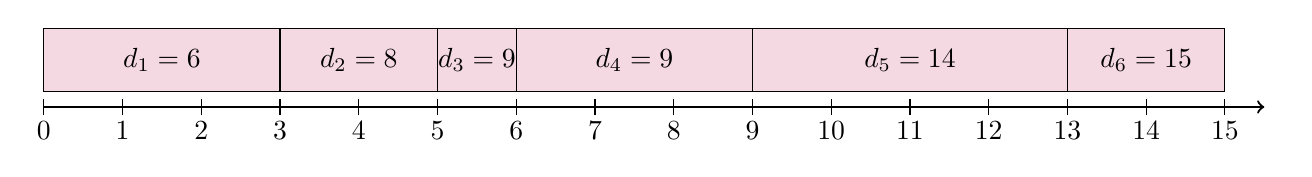
\begin{tikzpicture}
        % Draw the timeline
        \draw[thick,->] (0,0) -- (15.5,0) node[right] {};
        
        % Labels for time points
        \foreach \x in {0, 1, 2, 3, 4, 5, 6, 7, 8, 9, 10, 11, 12, 13, 14, 15} {
            \draw (\x,0.1) -- (\x,-0.1);
            \node at (\x,-0.3) {\x};
        }
        
        % Rectangles for jobs
        \filldraw[fill=purple!15] (0,0.2) rectangle (3,1);
        \node at (1.5,0.6) {$d_1 = 6$};
    
        \filldraw[fill=purple!15] (3,0.2) rectangle (5,1);
        \node at (4,0.6) {$d_2 = 8$};
    
        \filldraw[fill=purple!15] (5,0.2) rectangle (6,1);
        \node[inner sep=3pt] at (5.5,0.6) {$d_3 = 9$};
    
        \filldraw[fill=purple!15] (6,0.2) rectangle (9,1);
        \node at (7.5,0.6) {$d_4 = 9$};
    
        \filldraw[fill=purple!15] (9,0.2) rectangle (13,1);
        \node at (11,0.6) {$d_5 = 14$};
    
        \filldraw[fill=purple!15] (13,0.2) rectangle (15,1);
        \node at (14,0.6) {$d_6 = 15$};
        
    \end{tikzpicture}
    \caption{Where our number line represents time, and the rectangles the interval of each job.}
    \label{tab:late_sol}
\end{figure}

\noindent
Here we observe that we at most have $1$ late job.

